\setchapterimage[3.5cm]{mma/crab-page}
\setchapterpreamble[u]{\margintoc}
\chapter{Multi-Messenger Astronomy}
\labch{theory}
\begin{fquote}[William Shakespeare][Hamlet][1556] Though this be madness, yet there is method in it.
\end{fquote}

Multi-wavelength astronomy seeks to understand the universe through correlations between photons of different energies. Multi-messenger astronomy expands this concept to incorporate information from non-photon messengers, namely cosmic rays, gravitational waves and neutrinos. Each messenger provides a unique view of astrophysical processes in objects.

\section{Photons}

\begin{marginfigure}
	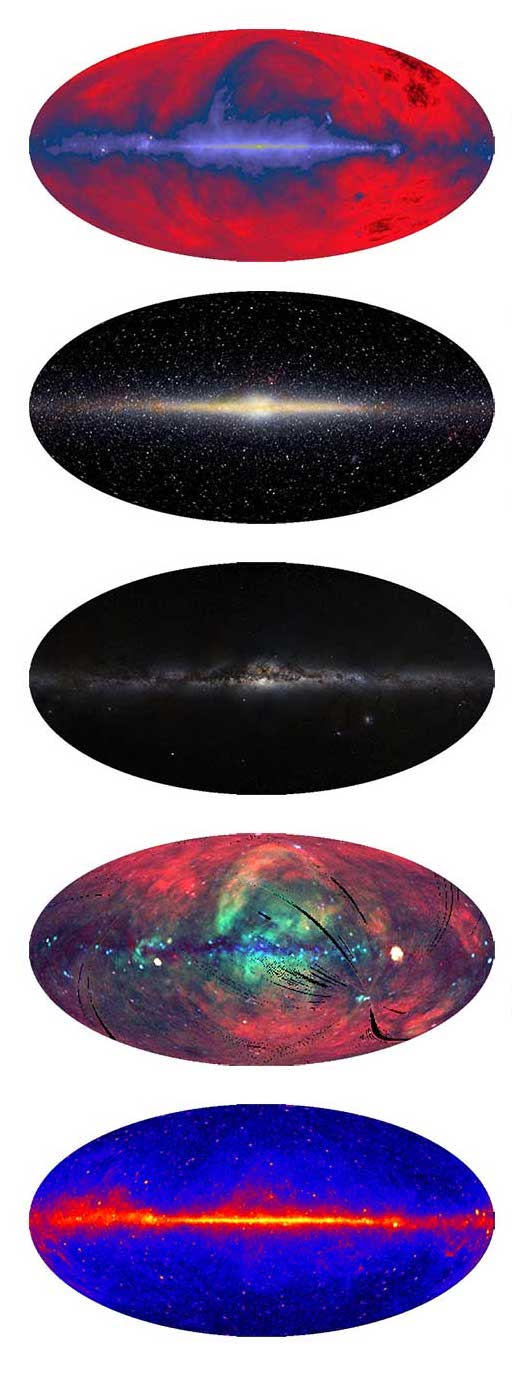
\includegraphics{mma/multiwavelength_sky_full}
	\caption{The sky, in galactic coordinates. From top: radio, infra-red, optical, X-ray and gamma-ray. Credit: NASA}
	\label{fig:mwsky}
\end{marginfigure}

Photon astronomy, in particular that in optical wavelengths, is the oldest branch of astronomy. As clear in Figure \ref{fig:mwsky}, our own galaxy is the most obvious structure at all wavelengths. The different pictures of the galaxy are also noteworthy. One example is dust extinction obscuring a large portion of the optical emission (middle panel), but  which is reprocessed to yield a particularly clear infra-red image (upper middle panel). This is an illustration of one broader principle, that interpolation between different photon energies can reveal .

In general, photon emission can be divided into two broad classes, \emph{thermal emission}
 and \emph{non-thermal emission}. Thermal emission is approximate black-bodies, and produces characteristic spectra. Non-thermal emission arises from particle acceleration, and is typically characterised by power-law emission. Objects can have both components. Thermal emission is typically centered in IR, optical or UV wavelengths, while non-thermal emission is typically manifested in both low energies (radio) and high-energies (hard X-rays and gamma-rays).
 
 \subsection*{Thermal Photons}

 \subsection*{Non-thermal Photons}
 
 \subsection*{Spectroscopy}
 
While photon observations are typically integrated over relatively-wide rsange of wavelengths, additional information can be gleaned from \emph{high-resolution spectroscopy}, in which emission in fine wavelength bins can be analysed. With precision measurements  

photoelectric effect?

\section{Cosmic Rays}

\emph{Cosmic Rays} were first discovered by Victor Hess in 1912 \sidecite{Hess:1912srp}. The name itself is a misnomer, as they are in fact charged particles. Being charged particles, they are deflected by magnetic fields, and it is thus challenging to determine where they originate from.

An industry of experiments has since developed to measure the composition and spectrum of Cosmic Rays, as illustrated in Figure \ref{fig:CR_spectrum}. The data is well-described by an unbroken power-law up to $\sim$1 PeV, beyond which there is a spectral softening known as \emph{the knee}. This softer spectrum continues before undergoing a hardening, known as the \emph{ankle}. There is then evidence of a high-energy cutoff, sometimes dubbed \emph{the second knee} in a case of metaphor-stretching.

\begin{figure}[!ht]
	\centering 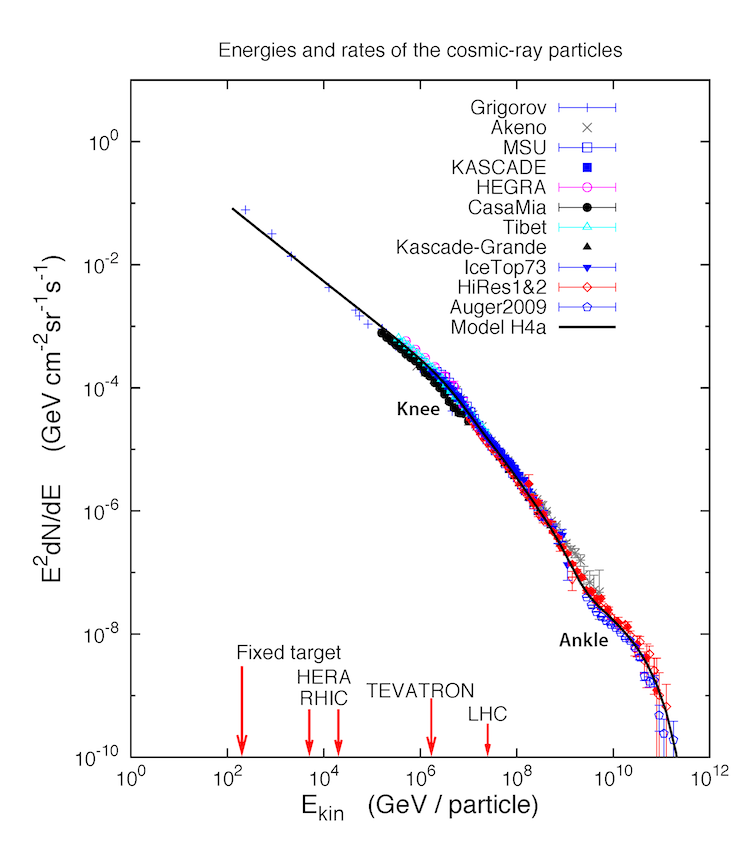
\includegraphics{mma/CRspectrum750}
	\caption{Cosmic Ray spectrum above 100 GeV, from x (icecube).}
	\label{fig:CR_spectrum}
\end{figure}

The knee is typically identified as the point at which cosmic rays transition from being predominantly galactic to extragalactic, with the ankle component being fully extragalactic. The origin of the high-energy cutoff is unclear, and the corresponding flux is so low that detector arrays must be several hundred square kilometers to study this regime with high statistics. As of 2020, this is primarily studied by the \emph{Pierre Auger Detector} and \emph {Telescope Array} detector. This regime is particularly interesting, because it is the point at which the GZK... mechanism 

UHECRs

\begin{equation}
p + \gamma_{CMB} \rightarrow \Delta^{+} \rightarrow n + \pi^{+}
\label{eq:GZK_pip}
\end{equation}
\begin{equation}
p + \gamma_{CMB} \rightarrow \Delta^{+} \rightarrow p + \pi^{0}
\label{eq:GZK_pi0}
\end{equation}

Equations \ref{eq:GZK_pip} and \ref{eq:GZK_pi0} would lead to a cutoff, in which pion production would suppress ultra-high energies above a threshold energy set by the mass of the $\Delta^{+}$ resonance. Attenuation would not occur for nearby cosmic ray sources, so the presence of such a cutoff would be evidence of an \emph{an extragalatic origin} for UHECRs. However, the \emph{Cosmic Ray Composition} determines the exact threshold for the GZK cutoff, with heavier comsic rays experiencing a much higher? threshold. There is thus much focus on understanding whether UHECRs are proton-dominated or Iron-dominated, with TA data supporting the former and PAO data supporting the latter. A joint working group concluded that these results are not in tension, once systematic uncertainties are accounted for. In summary, it appears that a definitive confirmation of a cutoff compatible with the GZK mechanism remains out of reach of present-generation instruments.

An alternative explanation for any apparent cutoff is that sources of UHECRs simply cannot accelerate particles beyond certain energies due to physical constraints. In general, any cosmic ray accelerator must at a minimum satisfy the \emph{Hillas Criterion} that any particle can be contained during the acceleration process \sidecite{1984ARA&A..22..425H}. This can be calculated by equating the Lamour Radius of a particle with the physical size of an accelerator:

Enu?

\begin{equation}
\frac{E_{\textup{max}}}{\textup{PeV}} \approx
1600 \times \frac{B}{\textup{Gauss}} \times \frac{R}{10^{16} \textup{cm}} \times
\beta Z
\label{eq:hillas}
\end{equation}

Equation \ref{eq:hillas} leads to a constraint on minimal magnetic field strength and source extension, which can be illustrated by a \emph{Hillas Plot} such as that in Figure \ref{fig:hillas_plot}. 

\begin{figure}[!ht]
	\centering 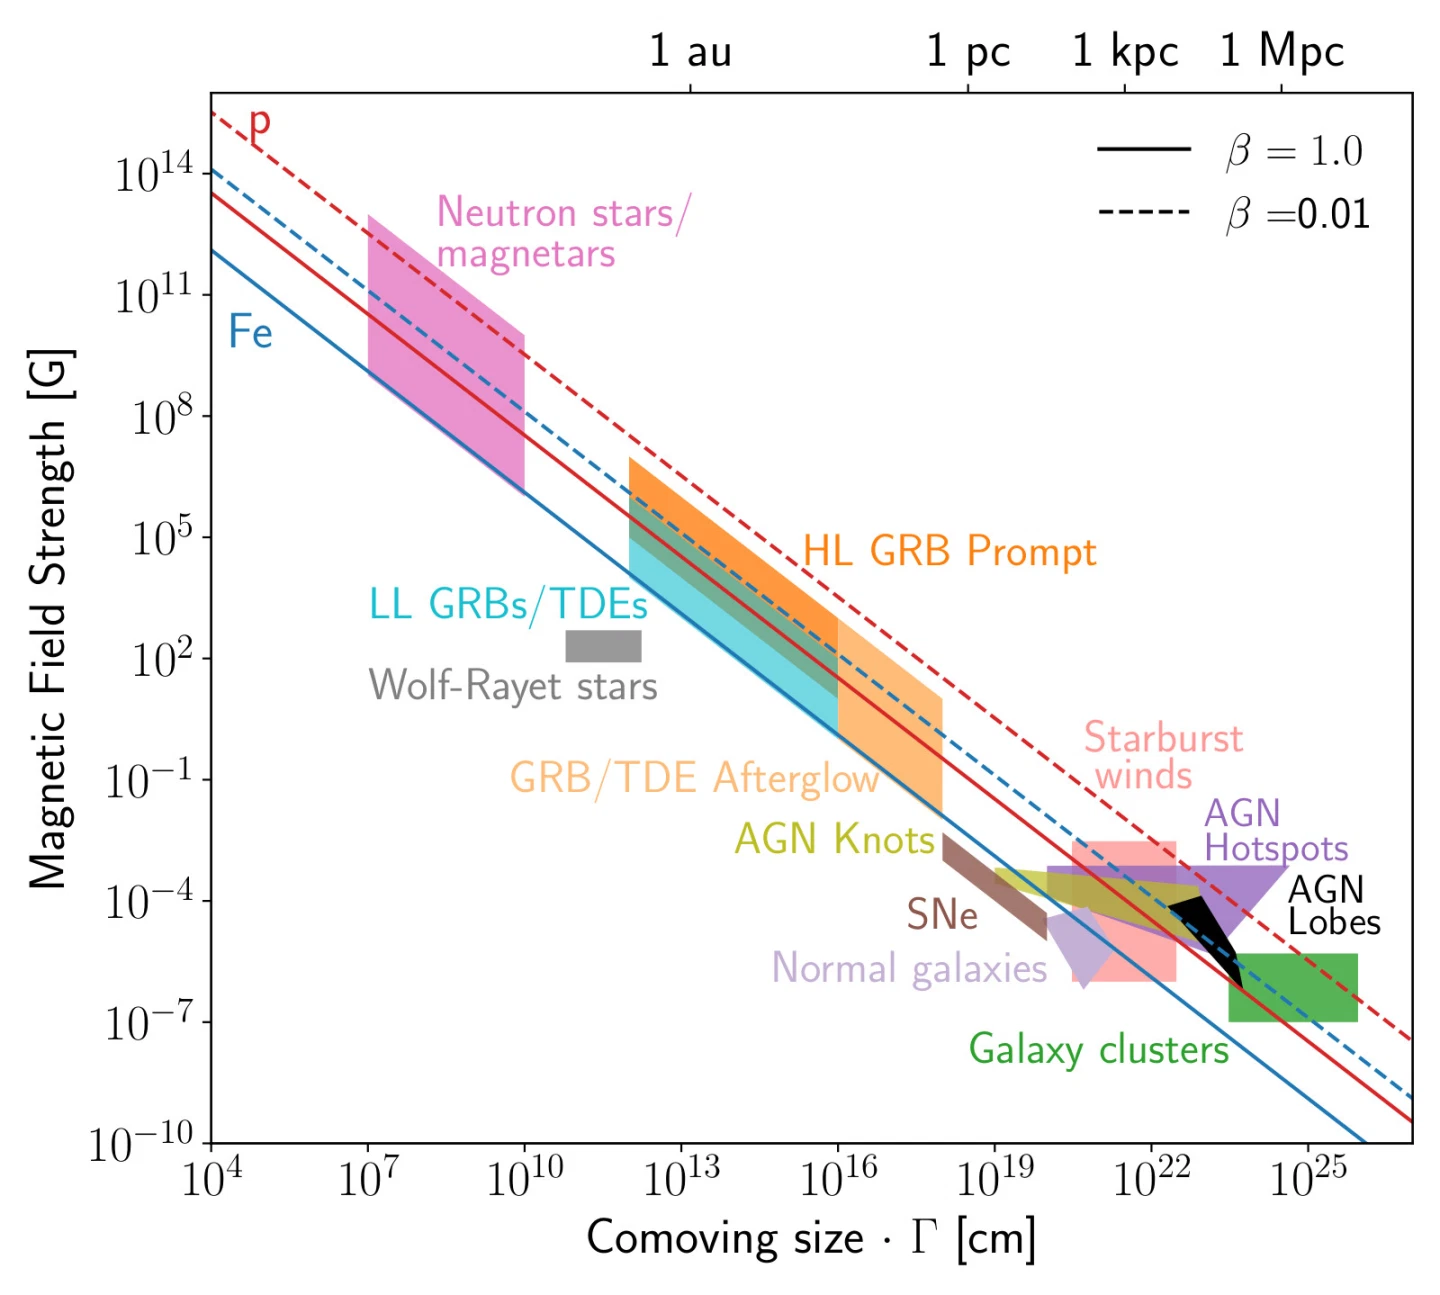
\includegraphics{mma/hillas}
	\caption{A Hillas plot illustrating possible cosmic-ray accelerators. credit: Mauricio B.}
	\label{fig:hillas_plot}
\end{figure}

The Hillas criterion \sidecite{1984ARA&A..22..425H} for a system of magnetic field strength $B$ and physical radius $R$ can be expressed as\cite{1984ARA&A..22..425H}:

\begin{equation}
\frac{E_{ \textup{max}}}{ \textup{PeV}} \approx
1600 \times \frac{B}{ \textup{Gauss}} \times \frac{R}{10^{16} \,  \textup{cm}} \times
\beta Z
\end{equation}
where $Z$ is the particle charge, $\beta \sim 0.2$ is the outflow velocity in units of c and $E$ is the maximum charged-particle energy. In order for particle acceleration to occur, the timescale required for particle acceleration must be shorter than the associated particle cooling timescale. Previous work has found this condition can be satisfied in TDEs for relevant energies\cite{2017ApJ...838....3S, 2017PhRvD..95l3001L}, although a detailed calculation is beyond the scope of this work.



Fermi acceleration

\section{Neutrinos}

The neutrino was first proposed as a particle by Pauli in 19xx as a solution to understand the mechanics of beta decay. Though observations suggested that the process involved a three-body decay, only the charged electron and proton could be measured. Invoking the existence of a light, chargeless particle provided a theoretical escape route. However, this particle was proven to be more than a theoretical construct, with the first evidence of observation by x in y.

cowan reines

DUMAND...

In parallel, the \emph{Standard Solar Model} was developed in 19xx, which correctly identified that the sun was powered by nuclear fusion. This model came with a firm prediction of a guaranteed flux of electron anti-neutrinos, \emph{solar neutrinos}, which would be produced in tandem with thermal radiation. However, the first attempt to measure the solar neutrino flux, by the Homestake experiment in 196x, found a flux that was only half the predicted level. This deficit, dubbed the \emph{solar neutrino problem}, was subsequently confirmed by many other experiments.

The solar neutrino problem was finally resolved in 200n, when the electron neutrino deficit was conclusively matched with a corresponding excess of muon neutrinos. This confirmed the presence of \emph{neutrino oscillations}, by which neutrinos can change flavour states. To undergo oscillations, neutrinos must have different non-zero mass states, in contrast to previous assumptions in the Standard Model of particle physics. 

A new generation of experiments have developed to probe neutrino flavour oscillations across a range of energies, baselines and channels. In general, \emph{reactor neutrinos} are used to probe electron neutrino disappearance, while solar neutrinos are used to probe muon neutrino appearance. Our current knowledge is summarised in N. Only the difference in squared masses can be probed by these experiments, so while it is known that mass states 1 and 2 have a difference of neV, and 13 $\sim$neV, the absolute ordering could be either \emph{Normal ordering} (m1<m2<m3) or \emph{inverted ordering} (m3<m1<m2). Directly measuring these masses remains a particle physics aim, with recent experiments such as KATRIN probing the sub-eV regime. IceCube has provided the first evidence of neutrino oscillations over astronomical baselines, with the detection of astrophysical tau neutrinos.

In 1987, experiments studying the solar neutrino problem unexpectedly measured a simultaneous excess in neutrinos. This detection occurred shortly before the discovery of a nearby supernova in the L? Magellanic Clouds, and coincided with the core-collapse of that supernova\sidecite{sn1987a_neutrino}. These \emph{supernova neutrinos} were the first that could be cleanly identified as arising from beyond our solar system, and confirmed the essential \emph{neutrino cooling} that is required during the stellar core collapse. This was also the first example of astronomy with multiple messengers. Only nearby galactic supernovae produce a sufficiently large flux to be clearly identified against this background. However, the predicted diffuse supernova neutrino background will soon be within reach of experiments.

Interactions of cosmic rays with the atmosphere produce a guaranteed flux of \emph{atmospheric neutrinos}, and this was finally confirmed observationally with the AMANDA detector in 200n. This flux extends over many orders of magnitude,. It is expected that there should be a distinct second \emph{atmospheric prompt} component of neutrinos, produced via charm quark in the atmosphere. However, this component has not yet been measured.

\emph{Astrophysical neutrinos} are to some degree guaranteed as a byproduct of high-energy cosmic ray production, resulting via pion production from the interaction of cosmic rays with ambient matter (pp) and radiation (p$\gamma$). However, the extent of astrophysical neutrino production depends very substantially on the conditions at cosmic ray accelerators, with high fluxes requiring abundant target material for pion production. A flux of astrophysical neutrinos was first discovered by IceCube in 2013, at a level close to the maximal one. This astrophysical component begins to dominate over the atmospheric neutrinos above n TeV. No neutrino source has yet been discovered, but possible sources of these astrosphysical neutrinos are discussed further in Chapter N.

At the very highest energies, it is expected that the impact of the GZK cutoff (Equations \ref{eq:GZK_pip} and \ref{eq:GZK_pi0}) should generate a flux of neutrinos through interactions of UHECRs with the cosmic microwave background. These \emph{Cosmogenic Neutrinos} have not yet been observed, but upcoming radio neutrino observatories in particular are seeking to measure them. The flux of cosmogenic neutrinos depends very strongly on the composition, density and evolution of cosmic ray sources, so it remains unclear whether it will be accessible to these detectors. (See Fig N)

\begin{figure}[!ht]
	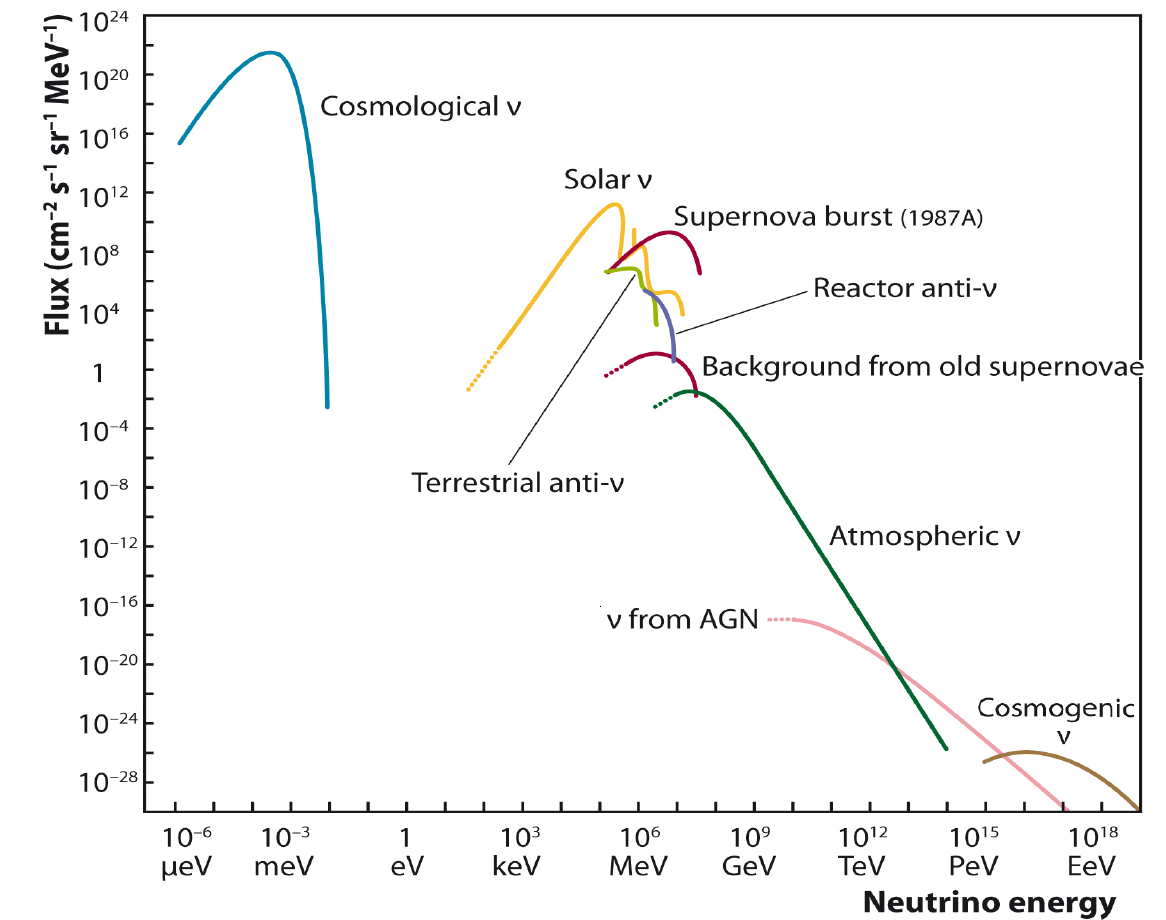
\includegraphics{mma/nu_spectrum}
	\caption{The full spectrum of neutrinos, from all sources. Credit: IceCube}
	\label{fig:nu_spectrum}
\end{figure}

\begin{figure}[!ht]
	\centering 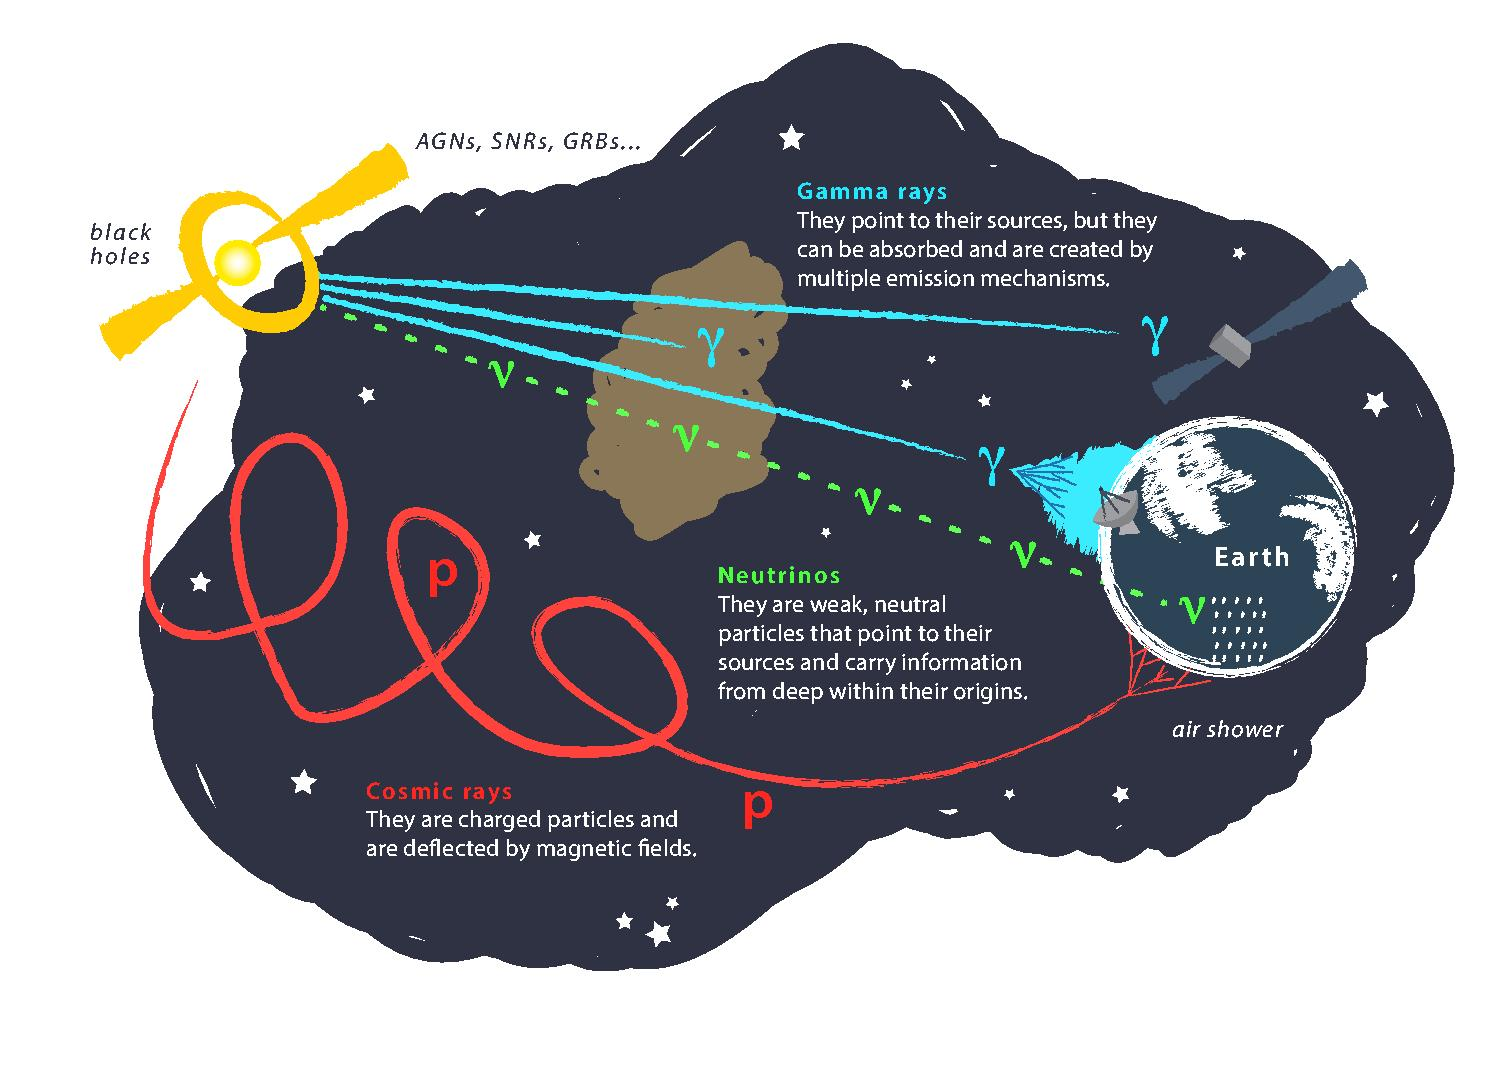
\includegraphics{mma/mm}
	\caption{An overview of multi-messenger astronomy. credit: IceCube.}
	\label{fig:mm}
\end{figure}

cosmological

In all cases, neutrino production is accompanied by a flux of pionic gamma-rays. However, these can be subsequently absorbed, so neutrinos may be produced in seemingly gamma-dark sources.

pp and p$\gamma$

For a photon target, with p$\gamma$ pion production via the $\Delta$ resonance, we expect that neutrino production will occur above the threshold introduced in Equation:

\begin{equation}
E_{\gamma}E_{p} \sim \Gamma ^{2} 0.16 \,  \textup{GeV}^{2}
\label{eq:delta_res}
\end{equation} 

Waxmann-Bachall.

glashow

MeV neutrinos from where? for ccsne
solar neutrino cycle

charged current
neutral current

\section{Gravitational Waves}

Einstein
LIGO
LISA
other sources?
quadropole moment
supernovae
Einstein Telescope
O4

The first indirect evidence for Gravitational waves came after the discovery of \emph{PSR J1915+1606}, the first pulsar binary \sidecite{hulse_taylor}. This binary system had an 8 hour orbital period that could be precisely measured in 1975, and could continue to be observed over the subsequent decades. The orbital period duration was seen to shorten over time, consistent with expectations from General Relativity for energy loss in the form of gravitational waves \sidecite{taylor_gr}. 

The arm length of gravitational waves determines 

An alternative method for direct gravitational wave detection also involves pulsars, namely the \emph{pulsar timing method} \sidecite{pulsar_gw_method}. In this case the `lever arm' is the distance to known pulsars, with passing gravitational waves being detected via the consequent deviation in pulsar cycles. The \emph{Interational Pulsar Timing Array} (IPTA) is the most comprehensive present effort to detect such emission, with sensitivity at x frequencies \sidecite{ipta}.

Recent NANOgrav results derived from pulsar timing could in principle be consistent with expectations for an astrophysical GW background, but no discovery has yet been claimed \sidecite{nanograv}.